\documentclass[a4paper, 12pt]{article}
\usepackage[swedish]{babel}
\usepackage[utf8]{inputenc}
\usepackage{verbatim}
\usepackage{fancyhdr}
\usepackage{graphicx}
\usepackage{parskip}
% Include pdf with multiple pages ex \includepdf[pages=-, nup=2x2]{filename.pdf}
\usepackage[final]{pdfpages}
% Place figures where they should be
\usepackage{float}

% vars
\def\title{Plugin 1.2}
\def\preTitle{Laboration 1}
\def\kurs{Applikationsprogrammering i Java, HT-08}

\def\namn{Anton Johansson}
\def\mail{dit06ajn@cs.umu.se}
\def\pathToCode{$\sim$dit06ajn/edu/apjava/lab1}

\def\handledareEtt{Johan Eliasson johane@cs.umu.se}
\def\inst{datavetenskap}
\def\dokumentTyp{Laborationsrapport}

\begin{document}
\begin{titlepage}
  \thispagestyle{empty}
  \begin{small}
    \begin{tabular}{@{}p{\textwidth}@{}}
      UMEÅ UNIVERSITET \hfill \today \\
      Institutionen för \inst \\
      \dokumentTyp \\
    \end{tabular}
  \end{small}
  \vspace{10mm}
  \begin{center}
    \LARGE{\preTitle} \\
    \huge{\textbf{\kurs}} \\
    \vspace{10mm}
    \LARGE{\title} \\
    \vspace{15mm}
    \begin{large}
        \namn, \mail \\
        \pathToCode
    \end{large}
    \vfill
    \large{\textbf{Handledare}}\\
    \mbox{\large{\handledareEtt}}
  \end{center}
\end{titlepage}

\pagestyle{fancy}
\rhead{\today}
\lhead{\namn, \mail}
\chead{}
\lfoot{}
\cfoot{}
\rfoot{}

\tableofcontents
\newpage

\rfoot{\thepage}
\pagenumbering{arabic}

\section{Problemspecifikation}
% Beskriv med egna ord vad uppgiften gick ut på. Är det någonting som
% varit oklart och ni gjort egna tolkningar så beskriv dessa.
Denna laboration gick ut på att skriva ett Javaprogram som använder
sig av Javas paket \textit{java.lang.reflect}. Paketet har funktioner
som gör det möjligt att inspektera, instansera, modifiera och exekvera
objekt och klasser medan ett program körs.

Till detta program skulle ett grafiskt gränssnitt skrivas. Från detta
grafiska gränssnitt kan metoder exekveras och eventuell utdata skrivs
ut på ett textfält.

Problemspecifikation finns i original på:\\
\verb!http://www.cs.umu.se/kurser/5DV085/HT08/labbar/lab1.html!

\section{Användarhandledning}
% Förklara var programmet och källkoden ligger samt hur man startar,
% kompilerar och använder det.
Programmet ligger i katalogen:\\
\pathToCode

Från denna katalog kompileras programmet med kommandot:

\verb!salt:~/edu/apjava/lab1> ant!

Källkoden ligger i underkatalogen \verb!src!.

Programmet tar vid start emot ett argument, detta ska vara namnet på
en klass som implementerar gränssnittet Plugable % TODO referens
och finns tillgängligt i aktuell classpath. För att köra programmet
med klassen \textit{Calc}:

\verb!salt:~/edu/apjava/lab1> java -cp bin/prod/ MyToolbox Calc!

Detta resulterar i följande grafiska gränssnitt:

\begin{figure}[H]
  \begin{center}
    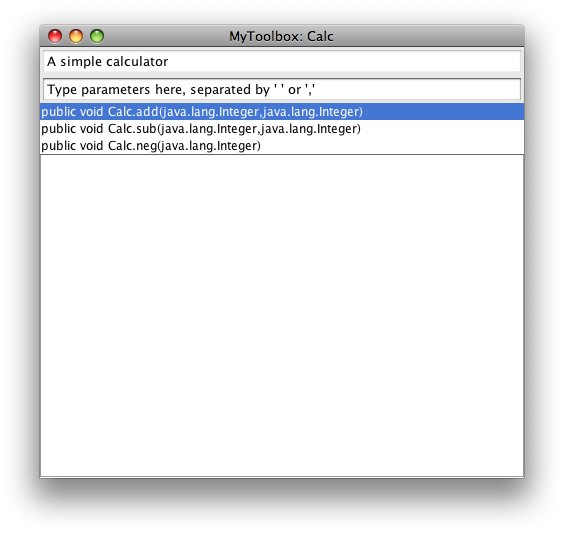
\includegraphics[width=110mm]{images/gui-out.png}
    \caption{GUI}
    \label{fig:gui}
  \end{center}
\end{figure}

I figur \ref{fig:gui} visar första fältet beskrivningen för klassen
\textit{Calc}. I nästa fält kan användaren ange parametrar som kan
behövas för att exekvera klassens metoder. I listan under vissas alla
metoder som är direkt deklarerade i klassen.

För att köra en metod fyller användaren i nödvändiga parametrar i
parameterfältet och trycker \verb!ENTER!, då körs markerad metod i
metodlistan. Alternativt kan användaren dubbelklicka på en metod, då
körs denna metod med de parametrar som finns ifyllda i
parameterfältet.

\section{Systembeskrivning}
% Beskriv översiktligt hur programmet är uppbyggt och hur det löser
% problemet.
Programmet består huvudsakligen av två klasser, \textit{MyToolbox} och
\textit{ClassHandler}. Klassen \textit{MyToolbox} startar programmet
och har ansvar för att rita det grafiska gränssnittet, klassen
kontrollerar även indata och utdata till och från användaren. I en
''Model-View-Controller''-design skulle klassen \textit{MyToolbox}
motsvara ''View-Controller''-delen. I samma modell motsvarar klassen
\textit{ClassHandler} ''Model''-delen, det vill säga det är i
\textit{ClassHandler} som programmet har sin grundfunktionalitet och
data.

\begin{figure}[H]
  \begin{center}
    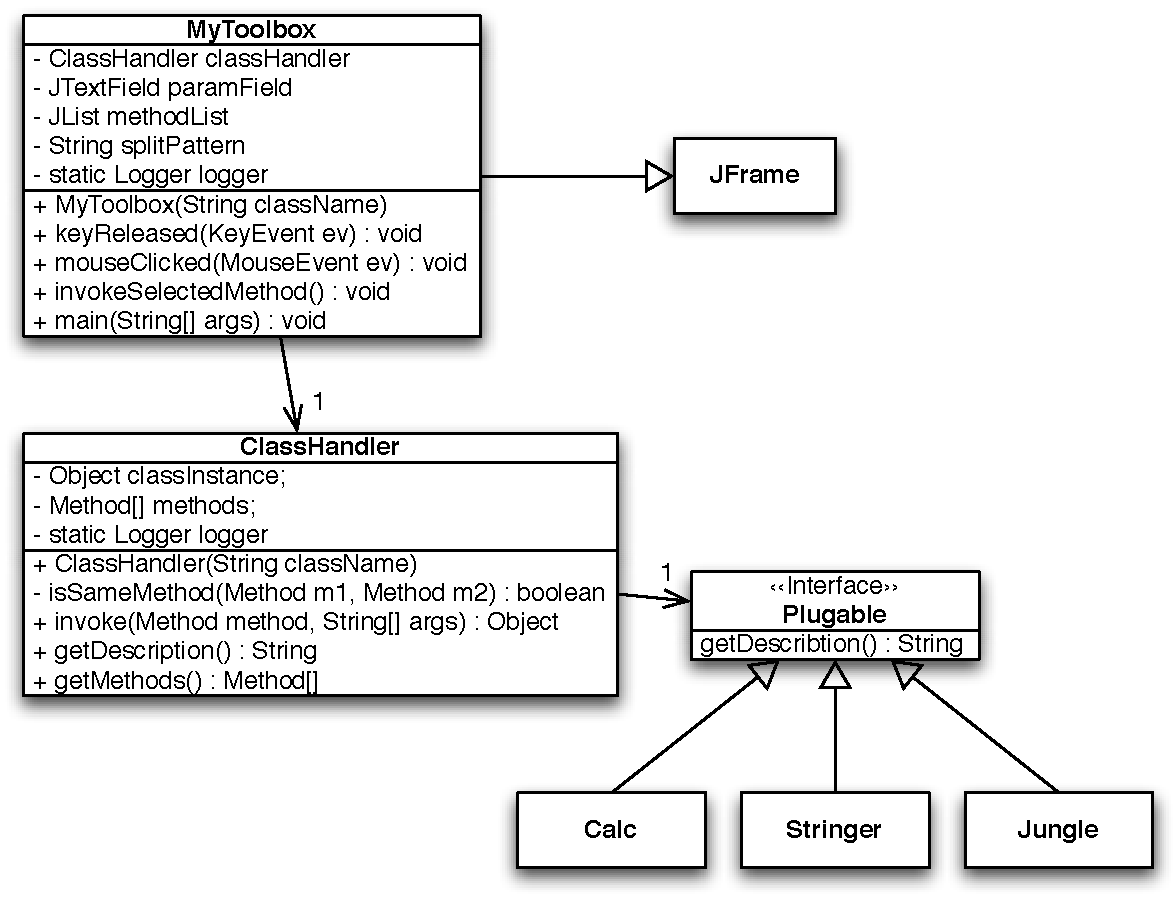
\includegraphics[width=130mm]{images/class.pdf}
    \caption{Klassdiagram}
    \label{fig:class}
  \end{center}
\end{figure}

\subsection{MyToolbox}
Klassen \textit{MyToolbox} ritar upp det grafiska gränssnittet genom
att ärva från klassen \textit{JFrame}. I klassens konstruktor skapas
en instans av klassen \textit{ClassHandler} och alla element som finns
i gränssnittet skapas och läggs in i paneler av typ
\textit{JPanel}. Lyssnare, Javas \textit{KeyAdapter} respektive
\textit{MouseAdapter}, kopplas till det grafiska fältet som tar emot
parametrar och listan som innehåller metoder. Dessa lyssnare har
metoder som reagerar på musklick och tangentbordstryck, när något av
detta händer så kommer vald metod att exekveras genom ett anrop till
klassen \textit{ClassHandler}. I \textit{main}-metoden som används för
att starta programmet fångas eventuella undantag som hindrar fortsatt
exekvering av programmet. Exempel på sådana undantag är om argumentet
som skickas med till MyToolbox inte är namnet på en klass som
återfinns vid körning, om denna klass inte implementerar
\textit{Plugable} eller om klassen inte har en standardkonstruktor
utan parametrar.

\subsection{ClassHandler}
Klassen \textit{ClassHandler} tar emot en textsträng i sin
konstruktor. Denna textsträng ska vara namnet på en klass som
implementerar gränssnittet Plugable och finns i aktuell classpath när
programmet körs. En ny instans av klassen med det medskickade namnet
skapas med hjälp av metoderna \textit{Class.forName()} och
\textit{Class.newInstance()} i Javas paket \textit{java.lang.reflect}.

Alla metoder deklarerade i den laddade klassen, som inte är
implementationer från gränssnittet \textit{Plugable}, sparas undan i ett
fält \textit{methods}. Metoder för att hämta och köra dessa metoder är
implementerade. Ytterligare finns en metod för att hämta en kort
beskrivning av den laddade klassen, denna metod anropar den laddade
klassens metod \textit{getDescription()} som är ett krav från
gränssnittet \textit{Plugable}.

\subsection{Plugable}
Gränssnittet \textit{Plugable} garanterar att klasserna som laddas in i
\textit{ClassHandler} har en metod \textit{getDescription()} som
returnerar en kort textsträng med en beskrivning av den laddade
klassens funktionalitet.

\section{Begränsningar}
% Vilka problem och begränsningar har din lösning av uppgiften? Hur
% skulle de kunna rättas till?

Eftersom man skickar in klassen när man kör programmet från terminalen
så sköts alla undantag i main metoden. Det erbjuds ingen möjlighet att
ändra eller korrigera klass i det grafiska gränssnittet. Hade det
grafiska gränssnittet kunnat hantera detta hade dessa try catch block
flyttats upp bland den koden.

Kravet på att klassen som laddas in i programmet ska implementera
gränssnittet \textit{Plugable} hade inte behövt vara så hårt, man
skulle lika gärna kunna ladda in vilken klass som helst, skillnaden
hade blivit att man inte fått något kort beskrivning av klassen.

% TODO - Vad händer om man laddar en klass utan metoder, inga
% relevanta felmeddelanden och det kan bli nullpointer

\section{Reflektioner}
% Var det något som var speciellt krångligt? Vilka problem uppstod och
% hur löste ni dem? Allmänna synpunkter. Hur skulle man kunna använda
% dessa metoder i andra mer omfattande system?

\section{Testkörningar}
%Noggranna testkörningar där man ser att programmet fungerar som det ska.

\section{Diskussion}
% Hur fungerade det att följa en kodkonvention? Vilka var fördelarna
% respektive nackdelarna?

\newpage
\appendix
\pagenumbering{arabic}
\section{Källkod}
% Källkoden ska finnas tillgänglig i er hemkatalog
% ~/edu/apjava/lab1/. Bifoga även utskriven källkod. Rekommenderat är
% att ni skriver ut den med kommandot
\subsection{MyToolbox.java}
\begin{footnotesize}
\verbatiminput{../src/MyToolbox.java}
\end{footnotesize}

\subsection{ClassHandler.java}
\begin{footnotesize}
\verbatiminput{../src/ClassHandler.java}
\end{footnotesize}

\subsection{Plugable.java}
\begin{footnotesize}
\verbatiminput{../src/Plugable.java}
\end{footnotesize}

\subsection{Jungle.java}
\begin{footnotesize}
\verbatiminput{../src/Jungle.java}
\end{footnotesize}

\end{document}
